\documentclass{article}

\usepackage[utf8]{inputenc}
\usepackage[letterpaper, total={6in, 9in}]{geometry}
\usepackage{amsmath}
\usepackage{natbib}
\usepackage{wrapfig}
\usepackage{graphicx}
\usepackage{amssymb}
\usepackage{tikz}

\title{Geometry 4 - Analytic Geomtry}
\author{TSS Math Club}
\date{Nov 2022}

\begin{document}
\large

\maketitle

\section{Preliminary}

% \subsection{Field}

% \subsubsection{Definition}

% \begin{itemize}
%     \item Associativity of addition and multiplication:
%     \item Commutativity of addition and multiplication:
%     \item Additive and multiplicative identity:
%     \item Additive inverses:
%     \item Multiplicative inverses:
%     \item Distributivity of multiplication over addition:
% \end{itemize}

\subsection{Real Line}

\subsubsection{Definition}

A number line is a picture of a graduated straight line that serves as visual representation of the real numbers. Every point of a number line is assumed to correspond to a real number, and every real number to a point.



\tikzset{every picture/.style={line width=0.75pt}} %set default line width to 0.75pt        

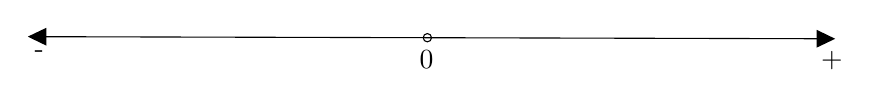
\begin{tikzpicture}[x=0.75pt,y=0.75pt,yscale=-1,xscale=1]
%uncomment if require: \path (0,411); %set diagram left start at 0, and has height of 411

%Straight Lines [id:da37370818120152194] 
\draw    (103,122.01) -- (486.01,123.02) ;
\draw [shift={(489.01,123.03)}, rotate = 180.15] [fill={rgb, 255:red, 0; green, 0; blue, 0 }  ][line width=0.08]  [draw opacity=0] (8.93,-4.29) -- (0,0) -- (8.93,4.29) -- cycle    ;
\draw [shift={(100,122)}, rotate = 0.15] [fill={rgb, 255:red, 0; green, 0; blue, 0 }  ][line width=0.08]  [draw opacity=0] (8.93,-4.29) -- (0,0) -- (8.93,4.29) -- cycle    ;
%Shape: Circle [id:dp6550024446713398] 
\draw   (290.52,122.51) .. controls (290.52,121.41) and (291.41,120.52) .. (292.51,120.52) .. controls (293.62,120.52) and (294.51,121.41) .. (294.51,122.51) .. controls (294.51,123.61) and (293.62,124.51) .. (292.51,124.51) .. controls (291.41,124.51) and (290.52,123.61) .. (290.52,122.51) -- cycle ;

% Text Node
\draw (287.51,127.51) node [anchor=north west][inner sep=0.75pt]   [align=left] {0};
% Text Node
\draw (481,128) node [anchor=north west][inner sep=0.75pt]   [align=left] {+};
% Text Node
\draw (102,125) node [anchor=north west][inner sep=0.75pt]   [align=left] {\mbox{-}};


\end{tikzpicture}


\subsection{Ordered Pair}

\subsubsection{Definition}

Informal:
\begin{quote}
For any two objects a and b, the ordered pair (a, b) is a notation specifying the two objects a and b, in that order.
\end{quote}
Formal:
\begin{quote}
(a,b)=\{\{a\},\{a,b\}\}
\end{quote}

\subsubsection{Property}

$$(a,b)=(c,d) \iff a=c \land b=d$$

\subsection{Cartesian Product}

\subsubsection{Definition}

The Cartesian product of two sets $A$ and $B$, denoted $A \times B$, is the set of all ordered pairs $(a, b)$ where $a$ is in $A$ and $b$ is in $B$.

$$A \times B = \{(a,b) \mid a \in A, b \in B \}$$


\section{Cartesian Plane}

\subsection{Definition}
In Mathematics, the cartesian plane is defined as a two-dimensional coordinate plane, which is formed by the intersection of the x-axis and y-axis. The x-axis and y-axis intersect perpendicular to each other at the point called the origin.


\subsection{Visual Representation}



\tikzset{every picture/.style={line width=0.75pt}} %set default line width to 0.75pt        

\begin{tikzpicture}[x=0.75pt,y=0.75pt,yscale=-.7,xscale=.7]
%uncomment if require: \path (0,300); %set diagram left start at 0, and has height of 300

%Straight Lines [id:da5485385098063555] 
\draw    (256.01,257.03) -- (256.01,26.03) ;
\draw [shift={(256.01,24.03)}, rotate = 90] [color={rgb, 255:red, 0; green, 0; blue, 0 }  ][line width=0.75]    (10.93,-3.29) .. controls (6.95,-1.4) and (3.31,-0.3) .. (0,0) .. controls (3.31,0.3) and (6.95,1.4) .. (10.93,3.29)   ;
%Straight Lines [id:da9244581279454482] 
\draw    (95.01,161.03) -- (433.01,160.03) ;
\draw [shift={(435.01,160.03)}, rotate = 179.83] [color={rgb, 255:red, 0; green, 0; blue, 0 }  ][line width=0.75]    (10.93,-3.29) .. controls (6.95,-1.4) and (3.31,-0.3) .. (0,0) .. controls (3.31,0.3) and (6.95,1.4) .. (10.93,3.29)   ;




\end{tikzpicture}


\subsection{Point}
\subsubsection{Definition}
A point is a primitive notion that models an exact location in space, and has no length, width, or thickness. 

\subsubsection{Plot points}





\tikzset{every picture/.style={line width=0.75pt}} %set default line width to 0.75pt        

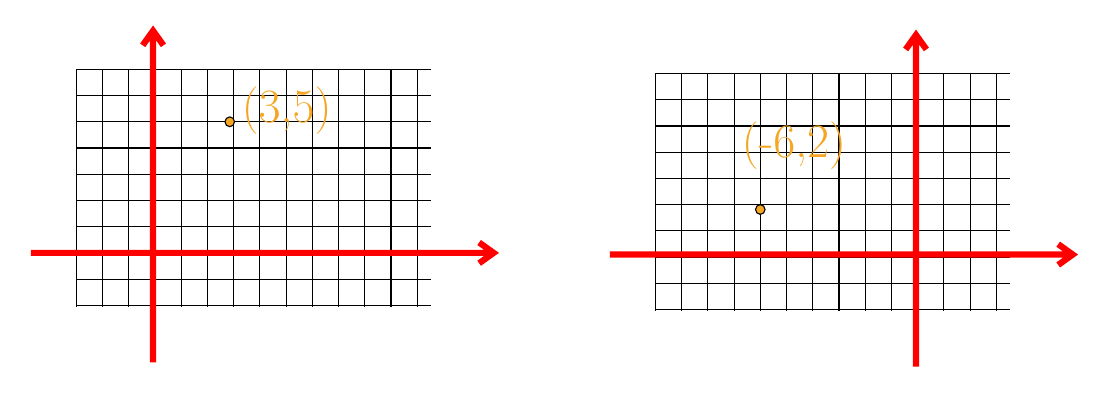
\begin{tikzpicture}[x=0.75pt,y=0.75pt,yscale=-1,xscale=1]
%uncomment if require: \path (0,300); %set diagram left start at 0, and has height of 300

%Shape: Grid [id:dp09064694594513245] 
\draw  [draw opacity=0] (58.64,106.92) -- (229.67,106.92) -- (229.67,221.25) -- (58.64,221.25) -- cycle ; \draw   (58.64,106.92) -- (58.64,221.25)(71.28,106.92) -- (71.28,221.25)(83.92,106.92) -- (83.92,221.25)(96.55,106.92) -- (96.55,221.25)(109.19,106.92) -- (109.19,221.25)(121.83,106.92) -- (121.83,221.25)(134.46,106.92) -- (134.46,221.25)(147.1,106.92) -- (147.1,221.25)(159.74,106.92) -- (159.74,221.25)(172.38,106.92) -- (172.38,221.25)(185.01,106.92) -- (185.01,221.25)(197.65,106.92) -- (197.65,221.25)(210.29,106.92) -- (210.29,221.25)(222.92,106.92) -- (222.92,221.25) ; \draw   (58.64,106.92) -- (229.67,106.92)(58.64,119.56) -- (229.67,119.56)(58.64,132.2) -- (229.67,132.2)(58.64,144.83) -- (229.67,144.83)(58.64,157.47) -- (229.67,157.47)(58.64,170.11) -- (229.67,170.11)(58.64,182.75) -- (229.67,182.75)(58.64,195.38) -- (229.67,195.38)(58.64,208.02) -- (229.67,208.02)(58.64,220.66) -- (229.67,220.66) ; \draw    ;
%Shape: Axis 2D [id:dp3391291012826534] 
\draw [color={rgb, 255:red, 255; green, 0; blue, 0 }  ,draw opacity=1 ][line width=2.25]  (36.72,195.35) -- (259.72,195.35)(95.64,88.35) -- (95.64,248.16) (252.72,190.35) -- (259.72,195.35) -- (252.72,200.35) (90.64,95.35) -- (95.64,88.35) -- (100.64,95.35)  ;
%Shape: Ellipse [id:dp767051254171291] 
\draw  [fill={rgb, 255:red, 245; green, 166; blue, 35 }  ,fill opacity=1 ] (130.29,132.2) .. controls (130.29,130.9) and (131.32,129.84) .. (132.58,129.84) .. controls (133.85,129.84) and (134.88,130.9) .. (134.88,132.2) .. controls (134.88,133.5) and (133.85,134.55) .. (132.58,134.55) .. controls (131.32,134.55) and (130.29,133.5) .. (130.29,132.2) -- cycle ;
%Shape: Grid [id:dp05039496198621474] 
\draw  [draw opacity=0] (337.64,108.92) -- (508.67,108.92) -- (508.67,223.25) -- (337.64,223.25) -- cycle ; \draw   (337.64,108.92) -- (337.64,223.25)(350.28,108.92) -- (350.28,223.25)(362.92,108.92) -- (362.92,223.25)(375.55,108.92) -- (375.55,223.25)(388.19,108.92) -- (388.19,223.25)(400.83,108.92) -- (400.83,223.25)(413.46,108.92) -- (413.46,223.25)(426.1,108.92) -- (426.1,223.25)(438.74,108.92) -- (438.74,223.25)(451.38,108.92) -- (451.38,223.25)(464.01,108.92) -- (464.01,223.25)(476.65,108.92) -- (476.65,223.25)(489.29,108.92) -- (489.29,223.25)(501.92,108.92) -- (501.92,223.25) ; \draw   (337.64,108.92) -- (508.67,108.92)(337.64,121.56) -- (508.67,121.56)(337.64,134.2) -- (508.67,134.2)(337.64,146.83) -- (508.67,146.83)(337.64,159.47) -- (508.67,159.47)(337.64,172.11) -- (508.67,172.11)(337.64,184.75) -- (508.67,184.75)(337.64,197.38) -- (508.67,197.38)(337.64,210.02) -- (508.67,210.02)(337.64,222.66) -- (508.67,222.66) ; \draw    ;
%Shape: Axis 2D [id:dp6799205357732412] 
\draw [color={rgb, 255:red, 255; green, 0; blue, 0 }  ,draw opacity=1 ][line width=2.25]  (315.72,196.16) -- (538.72,196.16)(463.23,90.35) -- (463.23,250.16) (531.72,191.16) -- (538.72,196.16) -- (531.72,201.16) (458.23,97.35) -- (463.23,90.35) -- (468.23,97.35)  ;
%Shape: Ellipse [id:dp5938164270153385] 
\draw  [fill={rgb, 255:red, 245; green, 166; blue, 35 }  ,fill opacity=1 ] (385.9,174.46) .. controls (385.9,173.16) and (386.92,172.11) .. (388.19,172.11) .. controls (389.46,172.11) and (390.48,173.16) .. (390.48,174.46) .. controls (390.48,175.76) and (389.46,176.81) .. (388.19,176.81) .. controls (386.92,176.81) and (385.9,175.76) .. (385.9,174.46) -- cycle ;

% Text Node
\draw (137.11,113.96) node [anchor=north west][inner sep=0.75pt]  [font=\LARGE,color={rgb, 255:red, 245; green, 166; blue, 35 }  ,opacity=1 ] [align=left] {(3,5)};
% Text Node
\draw (378.11,130.96) node [anchor=north west][inner sep=0.75pt]  [font=\LARGE,color={rgb, 255:red, 245; green, 166; blue, 35 }  ,opacity=1 ] [align=left] {(-6,2)};


\end{tikzpicture}


\subsection{Metric on the Plane}
\subsubsection{Distance formula}



\tikzset{every picture/.style={line width=0.75pt}} %set default line width to 0.75pt        

\begin{tikzpicture}[x=0.75pt,y=0.75pt,yscale=-.7,xscale=.7]
%uncomment if require: \path (0,300); %set diagram left start at 0, and has height of 300

%Straight Lines [id:da5485385098063555] 
\draw    (181.01,267.03) -- (181.01,36.03) ;
\draw [shift={(181.01,34.03)}, rotate = 90] [color={rgb, 255:red, 0; green, 0; blue, 0 }  ][line width=0.75]    (10.93,-3.29) .. controls (6.95,-1.4) and (3.31,-0.3) .. (0,0) .. controls (3.31,0.3) and (6.95,1.4) .. (10.93,3.29)   ;
%Straight Lines [id:da9244581279454482] 
\draw    (115.01,225.03) -- (453.01,224.03) ;
\draw [shift={(455.01,224.03)}, rotate = 179.83] [color={rgb, 255:red, 0; green, 0; blue, 0 }  ][line width=0.75]    (10.93,-3.29) .. controls (6.95,-1.4) and (3.31,-0.3) .. (0,0) .. controls (3.31,0.3) and (6.95,1.4) .. (10.93,3.29)   ;
%Straight Lines [id:da9012580532288677] 
\draw    (328.01,96.03) -- (228.01,174.03) ;

% Text Node
\draw (230.01,177.03) node [anchor=north west][inner sep=0.75pt]   [align=left] {(x1,y1)};
% Text Node
\draw (330.01,99.03) node [anchor=north west][inner sep=0.75pt]   [align=left] {(x2,y2)};


\end{tikzpicture}

$$d=\sqrt{(x_1-x_2)^2+(y_1-y_2)^2}$$

\subsubsection{Example}

Find the distance between (1,3) and (6,7).

$$d=\sqrt{(1-6)^2+(3-7)^2}=\sqrt{5^2+4^2}=\sqrt{41}$$

\subsection{Line}
\subsubsection{General Formula}
$$ax+by+c=0$$
\subsubsection{Examples}



\tikzset{every picture/.style={line width=0.75pt}} %set default line width to 0.75pt        

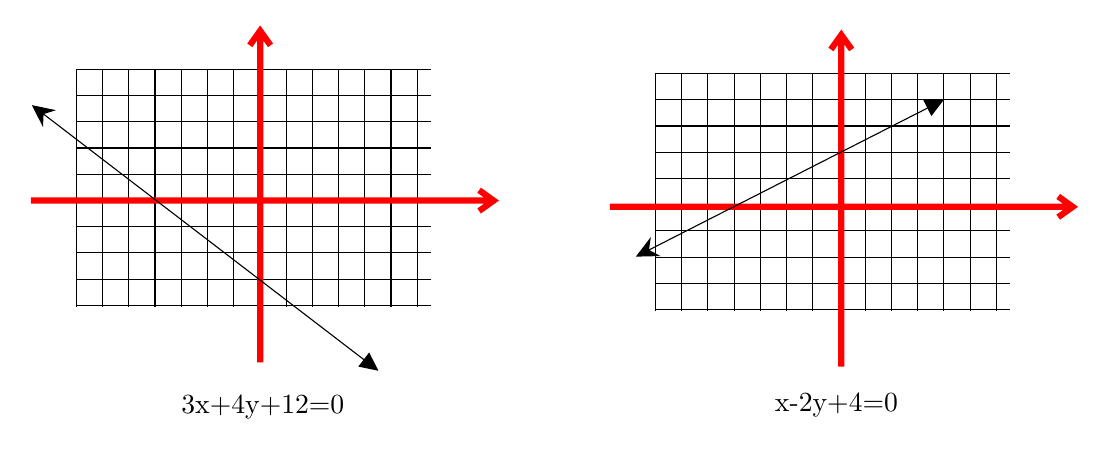
\begin{tikzpicture}[x=0.75pt,y=0.75pt,yscale=-1,xscale=1]
%uncomment if require: \path (0,337); %set diagram left start at 0, and has height of 337

%Shape: Grid [id:dp09064694594513245] 
\draw  [draw opacity=0] (58.64,106.92) -- (229.67,106.92) -- (229.67,221.25) -- (58.64,221.25) -- cycle ; \draw   (58.64,106.92) -- (58.64,221.25)(71.28,106.92) -- (71.28,221.25)(83.92,106.92) -- (83.92,221.25)(96.55,106.92) -- (96.55,221.25)(109.19,106.92) -- (109.19,221.25)(121.83,106.92) -- (121.83,221.25)(134.46,106.92) -- (134.46,221.25)(147.1,106.92) -- (147.1,221.25)(159.74,106.92) -- (159.74,221.25)(172.38,106.92) -- (172.38,221.25)(185.01,106.92) -- (185.01,221.25)(197.65,106.92) -- (197.65,221.25)(210.29,106.92) -- (210.29,221.25)(222.92,106.92) -- (222.92,221.25) ; \draw   (58.64,106.92) -- (229.67,106.92)(58.64,119.56) -- (229.67,119.56)(58.64,132.2) -- (229.67,132.2)(58.64,144.83) -- (229.67,144.83)(58.64,157.47) -- (229.67,157.47)(58.64,170.11) -- (229.67,170.11)(58.64,182.75) -- (229.67,182.75)(58.64,195.38) -- (229.67,195.38)(58.64,208.02) -- (229.67,208.02)(58.64,220.66) -- (229.67,220.66) ; \draw    ;
%Shape: Axis 2D [id:dp3391291012826534] 
\draw [color={rgb, 255:red, 255; green, 0; blue, 0 }  ,draw opacity=1 ][line width=2.25]  (36.72,170.16) -- (259.72,170.16)(147.23,88.35) -- (147.23,248.16) (252.72,165.16) -- (259.72,170.16) -- (252.72,175.16) (142.23,95.35) -- (147.23,88.35) -- (152.23,95.35)  ;
%Shape: Grid [id:dp05039496198621474] 
\draw  [draw opacity=0] (337.64,108.92) -- (508.67,108.92) -- (508.67,223.25) -- (337.64,223.25) -- cycle ; \draw   (337.64,108.92) -- (337.64,223.25)(350.28,108.92) -- (350.28,223.25)(362.92,108.92) -- (362.92,223.25)(375.55,108.92) -- (375.55,223.25)(388.19,108.92) -- (388.19,223.25)(400.83,108.92) -- (400.83,223.25)(413.46,108.92) -- (413.46,223.25)(426.1,108.92) -- (426.1,223.25)(438.74,108.92) -- (438.74,223.25)(451.38,108.92) -- (451.38,223.25)(464.01,108.92) -- (464.01,223.25)(476.65,108.92) -- (476.65,223.25)(489.29,108.92) -- (489.29,223.25)(501.92,108.92) -- (501.92,223.25) ; \draw   (337.64,108.92) -- (508.67,108.92)(337.64,121.56) -- (508.67,121.56)(337.64,134.2) -- (508.67,134.2)(337.64,146.83) -- (508.67,146.83)(337.64,159.47) -- (508.67,159.47)(337.64,172.11) -- (508.67,172.11)(337.64,184.75) -- (508.67,184.75)(337.64,197.38) -- (508.67,197.38)(337.64,210.02) -- (508.67,210.02)(337.64,222.66) -- (508.67,222.66) ; \draw    ;
%Shape: Axis 2D [id:dp6799205357732412] 
\draw [color={rgb, 255:red, 255; green, 0; blue, 0 }  ,draw opacity=1 ][line width=2.25]  (315.72,173.16) -- (538.72,173.16)(427.23,90.35) -- (427.23,250.16) (531.72,168.16) -- (538.72,173.16) -- (531.72,178.16) (422.23,97.35) -- (427.23,90.35) -- (432.23,97.35)  ;
%Straight Lines [id:da5489466012785622] 
\draw    (39.61,125.99) -- (201.85,250.34) ;
\draw [shift={(204.23,252.16)}, rotate = 217.47] [fill={rgb, 255:red, 0; green, 0; blue, 0 }  ][line width=0.08]  [draw opacity=0] (8.93,-4.29) -- (0,0) -- (8.93,4.29) -- cycle    ;
\draw [shift={(37.23,124.16)}, rotate = 37.47] [fill={rgb, 255:red, 0; green, 0; blue, 0 }  ][line width=0.08]  [draw opacity=0] (10.72,-5.15) -- (0,0) -- (10.72,5.15) -- (7.12,0) -- cycle    ;
%Straight Lines [id:da19183252165136278] 
\draw    (330.9,195.8) -- (473.98,122.92) ;
\draw [shift={(476.65,121.56)}, rotate = 153.01] [fill={rgb, 255:red, 0; green, 0; blue, 0 }  ][line width=0.08]  [draw opacity=0] (8.93,-4.29) -- (0,0) -- (8.93,4.29) -- cycle    ;
\draw [shift={(328.23,197.16)}, rotate = 333.01] [fill={rgb, 255:red, 0; green, 0; blue, 0 }  ][line width=0.08]  [draw opacity=0] (10.72,-5.15) -- (0,0) -- (10.72,5.15) -- (7.12,0) -- cycle    ;

% Text Node
\draw (108,263) node [anchor=north west][inner sep=0.75pt]   [align=left] {3x+4y+12=0};
% Text Node
\draw (394,262) node [anchor=north west][inner sep=0.75pt]   [align=left] {x-2y+4=0};


\end{tikzpicture}


\subsection{Circle}

\subsubsection{General Formula}
$$(x-a)^2+(y-b)^2=r^2$$ or
$$x^2+y^2+ax+by+c=0$$
\subsubsection{Examples}
Example 1:\\
$x^2+2x+y^2+4x+2=0$\\
$x^2+2x+1+y^2+4x+4=3$\\
$(x+1)^2+(y+2)^2=(\sqrt{3})^2$


\tikzset{every picture/.style={line width=0.75pt}} %set default line width to 0.75pt        

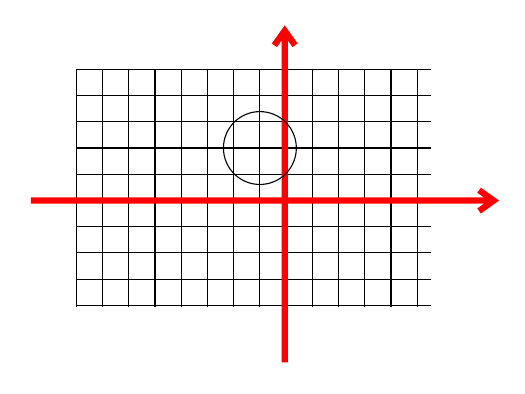
\begin{tikzpicture}[x=0.75pt,y=0.75pt,yscale=-1,xscale=1]
%uncomment if require: \path (0,337); %set diagram left start at 0, and has height of 337

%Shape: Grid [id:dp09064694594513245] 
\draw  [draw opacity=0] (58.64,106.92) -- (229.67,106.92) -- (229.67,221.25) -- (58.64,221.25) -- cycle ; \draw   (58.64,106.92) -- (58.64,221.25)(71.28,106.92) -- (71.28,221.25)(83.92,106.92) -- (83.92,221.25)(96.55,106.92) -- (96.55,221.25)(109.19,106.92) -- (109.19,221.25)(121.83,106.92) -- (121.83,221.25)(134.46,106.92) -- (134.46,221.25)(147.1,106.92) -- (147.1,221.25)(159.74,106.92) -- (159.74,221.25)(172.38,106.92) -- (172.38,221.25)(185.01,106.92) -- (185.01,221.25)(197.65,106.92) -- (197.65,221.25)(210.29,106.92) -- (210.29,221.25)(222.92,106.92) -- (222.92,221.25) ; \draw   (58.64,106.92) -- (229.67,106.92)(58.64,119.56) -- (229.67,119.56)(58.64,132.2) -- (229.67,132.2)(58.64,144.83) -- (229.67,144.83)(58.64,157.47) -- (229.67,157.47)(58.64,170.11) -- (229.67,170.11)(58.64,182.75) -- (229.67,182.75)(58.64,195.38) -- (229.67,195.38)(58.64,208.02) -- (229.67,208.02)(58.64,220.66) -- (229.67,220.66) ; \draw    ;
%Shape: Axis 2D [id:dp3391291012826534] 
\draw [color={rgb, 255:red, 255; green, 0; blue, 0 }  ,draw opacity=1 ][line width=2.25]  (36.72,170.16) -- (259.72,170.16)(159.06,88.35) -- (159.06,248.16) (252.72,165.16) -- (259.72,170.16) -- (252.72,175.16) (154.06,95.35) -- (159.06,88.35) -- (164.06,95.35)  ;
%Shape: Circle [id:dp5118138149603966] 
\draw   (129.54,144.83) .. controls (129.54,135.14) and (137.4,127.28) .. (147.1,127.28) .. controls (156.8,127.28) and (164.66,135.14) .. (164.66,144.83) .. controls (164.66,154.53) and (156.8,162.39) .. (147.1,162.39) .. controls (137.4,162.39) and (129.54,154.53) .. (129.54,144.83) -- cycle ;




\end{tikzpicture}\\\\
Example 2:


\tikzset{every picture/.style={line width=0.75pt}} %set default line width to 0.75pt        

\begin{tikzpicture}[x=0.75pt,y=0.75pt,yscale=-1,xscale=1]
%uncomment if require: \path (0,300); %set diagram left start at 0, and has height of 300

%Straight Lines [id:da40962903604479894] 
\draw    (401.93,207.03) -- (401.93,49.03) ;
\draw [shift={(401.93,47.03)}, rotate = 90] [color={rgb, 255:red, 0; green, 0; blue, 0 }  ][line width=0.75]    (10.93,-3.29) .. controls (6.95,-1.4) and (3.31,-0.3) .. (0,0) .. controls (3.31,0.3) and (6.95,1.4) .. (10.93,3.29)   ;
%Straight Lines [id:da02167311792978177] 
\draw    (302.01,141.1) -- (511.01,140.42) ;
\draw [shift={(513.01,140.42)}, rotate = 179.81] [color={rgb, 255:red, 0; green, 0; blue, 0 }  ][line width=0.75]    (10.93,-3.29) .. controls (6.95,-1.4) and (3.31,-0.3) .. (0,0) .. controls (3.31,0.3) and (6.95,1.4) .. (10.93,3.29)   ;
%Shape: Circle [id:dp6957597863561313] 
\draw   (423.97,94.01) .. controls (423.97,76.89) and (437.86,63) .. (454.99,63) .. controls (472.11,63) and (486,76.89) .. (486,94.01) .. controls (486,111.14) and (472.11,125.03) .. (454.99,125.03) .. controls (437.86,125.03) and (423.97,111.14) .. (423.97,94.01) -- cycle ;
%Straight Lines [id:da35029674067957206] 
\draw    (486.01,117.03) -- (456.59,95.2) ;
\draw [shift={(454.99,94.01)}, rotate = 36.56] [color={rgb, 255:red, 0; green, 0; blue, 0 }  ][line width=0.75]    (10.93,-3.29) .. controls (6.95,-1.4) and (3.31,-0.3) .. (0,0) .. controls (3.31,0.3) and (6.95,1.4) .. (10.93,3.29)   ;

% Text Node
\draw (486.99,108.01) node [anchor=north west][inner sep=0.75pt]   [align=left] {(3,4)};
% Text Node
\draw (485,69) node [anchor=north west][inner sep=0.75pt]   [align=left] {r=1};


\end{tikzpicture}\\
$(x-3)^2+(y-4)^2=1$ or $x^2 - 6 x + y^2 - 8 y + 24 = 0$

\subsection{Point to Line Distance Formula}

The distance between the line $ax+by+c = 0$ and point $(x_1,y_1)$ is\[\dfrac{|ax_1+by_1+c|}{\sqrt{a^2+b^2}}\]

\pagebreak


\subsection{Intersection}
\subsubsection{How to find intersection between two curve?}
Solve the system of equations.
\subsubsection{Example}

\tikzset{every picture/.style={line width=0.75pt}} %set default line width to 0.75pt        

\begin{tikzpicture}[x=0.75pt,y=0.75pt,yscale=-.8,xscale=.8]
%uncomment if require: \path (0,300); %set diagram left start at 0, and has height of 300

%Straight Lines [id:da40962903604479894] 
\draw    (259.01,280.03) -- (259.01,38.03) ;
\draw [shift={(259.01,36.03)}, rotate = 90] [color={rgb, 255:red, 0; green, 0; blue, 0 }  ][line width=0.75]    (10.93,-3.29) .. controls (6.95,-1.4) and (3.31,-0.3) .. (0,0) .. controls (3.31,0.3) and (6.95,1.4) .. (10.93,3.29)   ;
%Straight Lines [id:da02167311792978177] 
\draw    (98.01,179.49) -- (436.01,178.45) ;
\draw [shift={(438.01,178.45)}, rotate = 179.82] [color={rgb, 255:red, 0; green, 0; blue, 0 }  ][line width=0.75]    (10.93,-3.29) .. controls (6.95,-1.4) and (3.31,-0.3) .. (0,0) .. controls (3.31,0.3) and (6.95,1.4) .. (10.93,3.29)   ;
%Shape: Ellipse [id:dp6957597863561313] 
\draw   (309.54,102.68) .. controls (309.54,76.56) and (331.91,55.39) .. (359.51,55.39) .. controls (387.11,55.39) and (409.48,76.56) .. (409.48,102.68) .. controls (409.48,128.8) and (387.11,149.98) .. (359.51,149.98) .. controls (331.91,149.98) and (309.54,128.8) .. (309.54,102.68) -- cycle ;
%Straight Lines [id:da9711457273086297] 
\draw    (130.01,235.03) -- (444.01,9.03) ;

% Text Node
\draw (398,133) node [anchor=north west][inner sep=0.75pt]   [align=left] {(x-4)\textasciicircum 2+(y-3)\textasciicircum 2=2};
% Text Node
\draw (402,43) node [anchor=north west][inner sep=0.75pt]   [align=left] {2x-y=4};


\end{tikzpicture}\\
Sub $y=2x-4$ into $(x-4)^2+(y-3)^2=2$, \\
we get $(x-4)^2+(2x-4-3)^2=2$.\\
After solving, we get $x=3$ or $\frac{21}{5}.$\\
Therefore, the intersections are (3,2) and (21/5,22/5).


\subsubsection{Find the Radical Axis of Two Circles}
Definition: The line that passes through the intersections of the circles.\\
Find the radical axis bewteen $x^2+y^2=5$ and $x^2+3x+y^2-7y+3=0$.\\\\
Let P and Q be the intersection, Q and P must satisfy both $x^2+y^2=5$ and $x^2+3x+y^2-7y+3=0$, therefore the difference $3x-7y+3=-5$.\\
Since this line $ 3x-7y+8=0$ passes through P and Q, it must be the radical axis of two circles.




\pagebreak

\section{Vector}
\subsection{Definition}
"A quality that has both magnitude and direction."-physicist.\\
or an ordered pair (a,b)
\subsection{Visual Representation}


\tikzset{every picture/.style={line width=0.75pt}} %set default line width to 0.75pt        

\begin{tikzpicture}[x=0.75pt,y=0.75pt,yscale=-.7,xscale=.7]
%uncomment if require: \path (0,585); %set diagram left start at 0, and has height of 585

%Shape: Axis 2D [id:dp8227522849695434] 
\draw  (90,274.97) -- (381.72,274.97)(135.72,83.83) -- (135.72,313.97) (374.72,269.97) -- (381.72,274.97) -- (374.72,279.97) (130.72,90.83) -- (135.72,83.83) -- (140.72,90.83)  ;
%Straight Lines [id:da6629542579141938] 
\draw    (135.72,274.97) -- (251.04,201.05) ;
\draw [shift={(252.72,199.97)}, rotate = 147.34] [color={rgb, 255:red, 0; green, 0; blue, 0 }  ][line width=0.75]    (10.93,-3.29) .. controls (6.95,-1.4) and (3.31,-0.3) .. (0,0) .. controls (3.31,0.3) and (6.95,1.4) .. (10.93,3.29)   ;

% Text Node
\draw (250,183.83) node [anchor=north west][inner sep=0.75pt]   [align=left] {(a,b)};


\end{tikzpicture}

\subsection{Addition, Substraction and Scalar Multiplication of Vectors}
\subsubsection{Addition of Vectors}
Algebra: $(a,b)+(c,d)=(a+c,b+d)$\\
Geometry:



\tikzset{every picture/.style={line width=0.75pt}} %set default line width to 0.75pt        

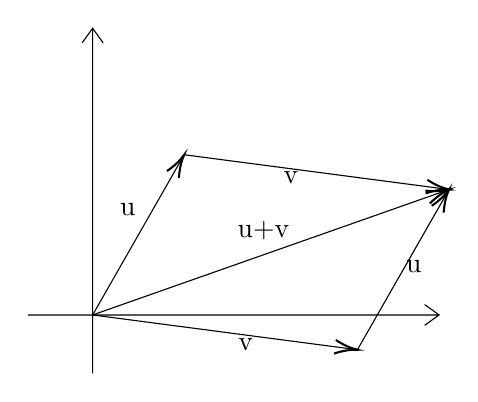
\begin{tikzpicture}[x=0.75pt,y=0.75pt,yscale=-1,xscale=1]
%uncomment if require: \path (0,585); %set diagram left start at 0, and has height of 585

%Shape: Axis 2D [id:dp8227522849695434] 
\draw  (90,221.97) -- (287.97,221.97)(121.03,83.83) -- (121.03,250.16) (280.97,216.97) -- (287.97,221.97) -- (280.97,226.97) (116.03,90.83) -- (121.03,83.83) -- (126.03,90.83)  ;
%Straight Lines [id:da6629542579141938] 
\draw    (121.03,221.97) -- (164.15,146.51) ;
\draw [shift={(165.14,144.78)}, rotate = 119.74] [color={rgb, 255:red, 0; green, 0; blue, 0 }  ][line width=0.75]    (10.93,-3.29) .. controls (6.95,-1.4) and (3.31,-0.3) .. (0,0) .. controls (3.31,0.3) and (6.95,1.4) .. (10.93,3.29)   ;
%Straight Lines [id:da9375942755586781] 
\draw    (121.03,221.97) -- (246.63,238.47) ;
\draw [shift={(248.61,238.73)}, rotate = 187.48] [color={rgb, 255:red, 0; green, 0; blue, 0 }  ][line width=0.75]    (10.93,-3.29) .. controls (6.95,-1.4) and (3.31,-0.3) .. (0,0) .. controls (3.31,0.3) and (6.95,1.4) .. (10.93,3.29)   ;
%Straight Lines [id:da4798526727664101] 
\draw    (165.14,144.78) -- (290.74,161.28) ;
\draw [shift={(292.72,161.54)}, rotate = 187.48] [color={rgb, 255:red, 0; green, 0; blue, 0 }  ][line width=0.75]    (10.93,-3.29) .. controls (6.95,-1.4) and (3.31,-0.3) .. (0,0) .. controls (3.31,0.3) and (6.95,1.4) .. (10.93,3.29)   ;
%Straight Lines [id:da485626268479008] 
\draw    (248.61,238.73) -- (291.73,163.28) ;
\draw [shift={(292.72,161.54)}, rotate = 119.74] [color={rgb, 255:red, 0; green, 0; blue, 0 }  ][line width=0.75]    (10.93,-3.29) .. controls (6.95,-1.4) and (3.31,-0.3) .. (0,0) .. controls (3.31,0.3) and (6.95,1.4) .. (10.93,3.29)   ;
%Straight Lines [id:da5449315364612841] 
\draw    (121.03,221.97) -- (290.83,162.2) ;
\draw [shift={(292.72,161.54)}, rotate = 160.61] [color={rgb, 255:red, 0; green, 0; blue, 0 }  ][line width=0.75]    (10.93,-3.29) .. controls (6.95,-1.4) and (3.31,-0.3) .. (0,0) .. controls (3.31,0.3) and (6.95,1.4) .. (10.93,3.29)   ;

% Text Node
\draw (133.02,166.88) node [anchor=north west][inner sep=0.75pt]   [align=left] {u};
% Text Node
\draw (190.03,231.93) node [anchor=north west][inner sep=0.75pt]   [align=left] {v};
% Text Node
\draw (211.74,151.7) node [anchor=north west][inner sep=0.75pt]   [align=left] {v};
% Text Node
\draw (270.78,194.34) node [anchor=north west][inner sep=0.75pt]   [align=left] {u};
% Text Node
\draw (189.65,175.55) node [anchor=north west][inner sep=0.75pt]   [align=left] {u+v};


\end{tikzpicture}

\subsubsection{Substraction of Vectors}
Algebra:$(a,b)-(c,d)=(a-c,b-d)$ \\
Geometry:



\tikzset{every picture/.style={line width=0.75pt}} %set default line width to 0.75pt        

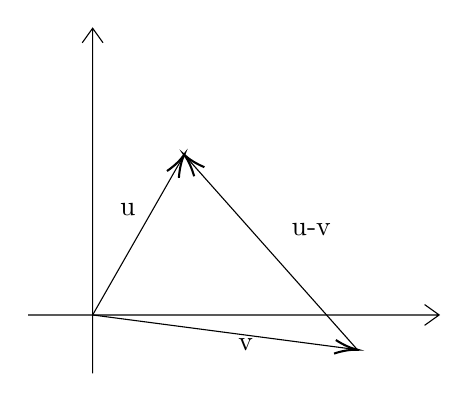
\begin{tikzpicture}[x=0.75pt,y=0.75pt,yscale=-1,xscale=1]
%uncomment if require: \path (0,585); %set diagram left start at 0, and has height of 585

%Shape: Axis 2D [id:dp8227522849695434] 
\draw  (90,221.97) -- (287.97,221.97)(121.03,83.83) -- (121.03,250.16) (280.97,216.97) -- (287.97,221.97) -- (280.97,226.97) (116.03,90.83) -- (121.03,83.83) -- (126.03,90.83)  ;
%Straight Lines [id:da6629542579141938] 
\draw    (121.03,221.97) -- (164.15,146.51) ;
\draw [shift={(165.14,144.78)}, rotate = 119.74] [color={rgb, 255:red, 0; green, 0; blue, 0 }  ][line width=0.75]    (10.93,-3.29) .. controls (6.95,-1.4) and (3.31,-0.3) .. (0,0) .. controls (3.31,0.3) and (6.95,1.4) .. (10.93,3.29)   ;
%Straight Lines [id:da9375942755586781] 
\draw    (121.03,221.97) -- (246.63,238.47) ;
\draw [shift={(248.61,238.73)}, rotate = 187.48] [color={rgb, 255:red, 0; green, 0; blue, 0 }  ][line width=0.75]    (10.93,-3.29) .. controls (6.95,-1.4) and (3.31,-0.3) .. (0,0) .. controls (3.31,0.3) and (6.95,1.4) .. (10.93,3.29)   ;
%Straight Lines [id:da5449315364612841] 
\draw    (248.61,238.73) -- (166.47,146.27) ;
\draw [shift={(165.14,144.78)}, rotate = 48.38] [color={rgb, 255:red, 0; green, 0; blue, 0 }  ][line width=0.75]    (10.93,-3.29) .. controls (6.95,-1.4) and (3.31,-0.3) .. (0,0) .. controls (3.31,0.3) and (6.95,1.4) .. (10.93,3.29)   ;

% Text Node
\draw (133.02,166.88) node [anchor=north west][inner sep=0.75pt]   [align=left] {u};
% Text Node
\draw (190.03,231.93) node [anchor=north west][inner sep=0.75pt]   [align=left] {v};
% Text Node
\draw (215.65,176.55) node [anchor=north west][inner sep=0.75pt]   [align=left] {u-v};


\end{tikzpicture}


\subsubsection{Scalar Multiplication of Vector}

Algebra: $c(a,b)=(ac,bc)$ \\
Geometry:


\tikzset{every picture/.style={line width=0.75pt}} %set default line width to 0.75pt        

\begin{tikzpicture}[x=0.75pt,y=0.75pt,yscale=-1,xscale=1]
%uncomment if require: \path (0,585); %set diagram left start at 0, and has height of 585

%Shape: Axis 2D [id:dp8227522849695434] 
\draw  (90,221.97) -- (287.97,221.97)(121.03,83.83) -- (121.03,250.16) (280.97,216.97) -- (287.97,221.97) -- (280.97,226.97) (116.03,90.83) -- (121.03,83.83) -- (126.03,90.83)  ;
%Straight Lines [id:da6629542579141938] 
\draw    (121.03,221.97) -- (164.15,146.51) ;
\draw [shift={(165.14,144.78)}, rotate = 119.74] [color={rgb, 255:red, 0; green, 0; blue, 0 }  ][line width=0.75]    (10.93,-3.29) .. controls (6.95,-1.4) and (3.31,-0.3) .. (0,0) .. controls (3.31,0.3) and (6.95,1.4) .. (10.93,3.29)   ;
%Straight Lines [id:da9375942755586781] 
\draw    (121.03,221.97) -- (186.71,109.89) ;
\draw [shift={(187.72,108.16)}, rotate = 120.37] [color={rgb, 255:red, 0; green, 0; blue, 0 }  ][line width=0.75]    (10.93,-3.29) .. controls (6.95,-1.4) and (3.31,-0.3) .. (0,0) .. controls (3.31,0.3) and (6.95,1.4) .. (10.93,3.29)   ;

% Text Node
\draw (133.02,166.88) node [anchor=north west][inner sep=0.75pt]   [align=left] {u};
% Text Node
\draw (148,124) node [anchor=north west][inner sep=0.75pt]   [align=left] {cu};


\end{tikzpicture}

\subsection{Dot Product}

\subsubsection{Definition: Dot Product on 2D}
If $x =(x_1,x_2)$ and $y=(y_1,y_2)$, then
$$x \cdot y = x_1y_1+x_2y_2$$

\subsubsection{Property: Dot Product}
\begin{itemize}
    \item positivity: $v\cdot v\ge 0$
    \item definiteness: $v\cdot v = 0$ iff $v=0$
    \item additivity: $(v+u)\cdot(w)=v\cdot w + u \cdot w$ or 
    \item homogeneity: $c(u\cdot v)=(cu)\cdot v$
    \item symmetry: $u \cdot v = v \cdot u$
\end{itemize}

\subsubsection{Dot Product and Metric}
$v\cdot v = |v|^2$

\subsubsection{Penpendicularity}
$v\cdot u=0$ if $v$ and $u$ are perpendicular to each other. 
\pagebreak

\subsubsection{Dot Product and Cosine Law}

\tikzset{every picture/.style={line width=0.75pt}} %set default line width to 0.75pt        

\begin{tikzpicture}[x=0.75pt,y=0.75pt,yscale=-1,xscale=1]
%uncomment if require: \path (0,585); %set diagram left start at 0, and has height of 585

%Straight Lines [id:da17404312810320866] 
\draw    (124.72,196.76) -- (243.1,91.49) ;
\draw [shift={(244.6,90.16)}, rotate = 138.35] [color={rgb, 255:red, 0; green, 0; blue, 0 }  ][line width=0.75]    (10.93,-3.29) .. controls (6.95,-1.4) and (3.31,-0.3) .. (0,0) .. controls (3.31,0.3) and (6.95,1.4) .. (10.93,3.29)   ;
%Straight Lines [id:da1385073769185674] 
\draw    (124.72,196.76) -- (374.74,230.34) ;
\draw [shift={(376.72,230.6)}, rotate = 187.65] [color={rgb, 255:red, 0; green, 0; blue, 0 }  ][line width=0.75]    (10.93,-3.29) .. controls (6.95,-1.4) and (3.31,-0.3) .. (0,0) .. controls (3.31,0.3) and (6.95,1.4) .. (10.93,3.29)   ;
%Straight Lines [id:da4938978023656899] 
\draw    (244.6,90.16) -- (375.35,229.15) ;
\draw [shift={(376.72,230.6)}, rotate = 226.75] [color={rgb, 255:red, 0; green, 0; blue, 0 }  ][line width=0.75]    (10.93,-3.29) .. controls (6.95,-1.4) and (3.31,-0.3) .. (0,0) .. controls (3.31,0.3) and (6.95,1.4) .. (10.93,3.29)   ;

% Text Node
\draw (167.15,131.86) node [anchor=north west][inner sep=0.75pt]   [align=left] {a};
% Text Node
\draw (236.28,214.78) node [anchor=north west][inner sep=0.75pt]   [align=left] {b};
% Text Node
\draw (317.72,148.79) node [anchor=north west][inner sep=0.75pt]   [align=left] {b-a};
% Text Node
\draw (148,179) node [anchor=north west][inner sep=0.75pt]   [align=left] {$\theta$};


\end{tikzpicture}\\
$$(b-a)\cdot(b-a)=b \cdot b+ a \cdot a - 2 a \cdot b$$
Compare with cosine law:
$$c^2=a^2+b^2-2ab\cos(C)$$
Therefore,
$$a\cdot b =|a||b|\cos(\theta)$$
\subsubsection{Dot Product as Projection}


\tikzset{every picture/.style={line width=0.75pt}} %set default line width to 0.75pt        

\begin{tikzpicture}[x=0.75pt,y=0.75pt,yscale=-1,xscale=1]
%uncomment if require: \path (0,585); %set diagram left start at 0, and has height of 585

%Straight Lines [id:da637575067913835] 
\draw    (133.72,284.16) -- (185.95,159.01) ;
\draw [shift={(186.72,157.16)}, rotate = 112.65] [color={rgb, 255:red, 0; green, 0; blue, 0 }  ][line width=0.75]    (10.93,-3.29) .. controls (6.95,-1.4) and (3.31,-0.3) .. (0,0) .. controls (3.31,0.3) and (6.95,1.4) .. (10.93,3.29)   ;
%Straight Lines [id:da6495955178480797] 
\draw    (133.72,284.16) -- (287.77,248.61) ;
\draw [shift={(289.72,248.16)}, rotate = 167.01] [color={rgb, 255:red, 0; green, 0; blue, 0 }  ][line width=0.75]    (10.93,-3.29) .. controls (6.95,-1.4) and (3.31,-0.3) .. (0,0) .. controls (3.31,0.3) and (6.95,1.4) .. (10.93,3.29)   ;
%Straight Lines [id:da8569645157359189] 
\draw  [dash pattern={on 0.84pt off 2.51pt}]  (186.72,157.16) -- (211.72,266.16) ;
%Straight Lines [id:da7064326740913383] 
\draw [color={rgb, 255:red, 255; green, 0; blue, 0 }  ,draw opacity=1 ]   (133.72,284.16) -- (209.77,266.61) ;
\draw [shift={(211.72,266.16)}, rotate = 167.01] [color={rgb, 255:red, 255; green, 0; blue, 0 }  ,draw opacity=1 ][line width=0.75]    (10.93,-3.29) .. controls (6.95,-1.4) and (3.31,-0.3) .. (0,0) .. controls (3.31,0.3) and (6.95,1.4) .. (10.93,3.29)   ;

% Text Node
\draw (145,196) node [anchor=north west][inner sep=0.75pt]   [align=left] {u};
% Text Node
\draw (228,267) node [anchor=north west][inner sep=0.75pt]   [align=left] {v};


\end{tikzpicture}\\
The projection of u on v is $$\frac{u \cdot v}{|v|}$$
\pagebreak
\subsubsection{Problem (1975 USAMO Q2)}
Let $A,B,C,D$ denote four points in space and $AB$ the distance between $A$ and $B$, and so on. Show that\[AC^2+BD^2+AD^2+BC^2\ge AB^2+CD^2.\]
Let $a$, $b$, $c$, $d$ correspond to the position vectors of points A, B, C, and D, respectively, with respect to an arbitrary origin O. Let us also for simplicity define $a^2 = a \cdot a = ||a||^2$, where $||a||$ is the magnitude of vector $a$. Because squares are non-negative, $a^2$ is non-negative for all vectors $a$. Thus,\[(a + b - c - d)^2 \ge 0\]Because dot product is linear, we expand to obtain\[a^2 + b^2 + c^2 + d^2 + 2a \cdot b + 2 c \cdot d - 2 a \cdot c - 2 a \cdot d - 2 b \cdot c - 2 c \cdot d \ge 0,\]from which we add $a^2 + b^2 + c^2 + d^2$ to both sides, rearrange, and complete the square to get\[(a-c)^2 + (a-d)^2 + (b-c)^2 + (b-d)^2 \ge (a-b)^2 + (c-d)^2.\]As $(a-b)^2 = ||a-b||^2 = ||AB||^2 = AB^2$ and likewise for the others,\[AC^2 + AD^2 + BC^2 + BD^2 \ge AB^2 + CD^2,\]which is what we wanted to prove.

\pagebreak

\subsection{Determinant}
\subsubsection{Definition}
The area of the parallelogram formed by 2 vectors, namely $(a,c)$ and $(b,d)$.
\subsubsection{Formula}

$
\begin{vmatrix}
    a & b\\
    c & d
\end{vmatrix}
= ad-bc
$

\subsubsection{3D Determinant and Area of a Triangle}
Definition:
The volume of the parallelepiped formed by 3 vectors, namely $(a,d,h), (b,e,i), (c,f,j)$.\\
Formula:
$$
\begin{vmatrix}
    a & b & c\\
    d & e & f\\
    h & i & j
\end{vmatrix}
=a
\begin{vmatrix}
   e  & f\\
   i  & j
\end{vmatrix}
-b
\begin{vmatrix}
   d  & f\\
   h  & j
\end{vmatrix}
+c
\begin{vmatrix}
   d  & e\\
   h  & i
\end{vmatrix}
$$
Area of a Triangle with Vertex $A(x_1,y_1), B(x_2,y_2), C(x_3,y_3)$ is 
$$
\begin{vmatrix}
    1 & 1 & 1\\
    x_1 & x_2 & x_3\\
    y_1 & y_2 & y_3
\end{vmatrix}
$$
\subsubsection{Shoelace Theorem}

Suppose the polygon $P$ has vertices $(a_1, b_1)$, $(a_2, b_2)$, ... , $(a_n, b_n)$, listed in clockwise order. Then the area ($A$) of $P$ is

\[A = \dfrac{1}{2} \left|\sum_{i=1}^n{\det\begin{pmatrix}x_i&x_{i+1}\\y_i&y_{i+1}\end{pmatrix}}\right|\]

\end{document}